%this is chapter about the process of benchmarking cardinality estimation for DBMS

\chapter{BENCHMARKING CARDINALITY ESTIMATION ON POSTGRESQL}\label{chapter:Benchmarking CE}
%this section is about basic theory used in this chapter
\section{BASIC THEORIES AND IMPORTANT CONCEPTS.}
%the definition of Q-error used to benchmark
\subsection{Q-error}
\subsubsection{The Definition of Q-error \cite{q-error}.}
{\justify
Let R be a relation and A be one of its attributes, and $\left\{x_{1},...,x_{m}\right\}$ = ${{\Pi}_{A}\left(R\right)}$ is the set of distinct values of A. Then, the frequency density is a set of pairs ${\left(x_{i},f_{i}\right)}$ with $f_{i}$ = $\vert{\sigma_{A=x_i}\left(R\right)}\vert$, ${{1}\le{i}\le{m}}$
\par }
\vspace{0.5cm}
{\justify
$F$ is a function to approximate this set of paris; $F\left(x_{i}\right)$ =: $F_{i}$ gives the estimate $F_{i}$ of $f_{i}$. And F is a polynomial of degree 0 or 1.
\par }
\vspace{0.5cm}
{\justify
Typically, norms are used to define the error. So, the correct values are organized into a vector $\vec{b}$ = ${{\left(f_{1},...,f_{m}\right)}^{T}}\in{{\mathbb{R}}^{m}}$ and the estimates into a vector $\vec{B}$ = ${{\left(F_{1},...,F_{m}\right)}^{T}}\in{{\mathbb{R}}^{m}}$. $l_{p}$ error metrics are based on $l_{p}$ norms as in 
\par }
{\centering ${\Vert{b-B}\Vert}_{p}$ \\}
{\justify
where ${{1}\le{p}\le{\infty}}$ and the most common norms are 
\par }
{\justify
\centering ${\Vert{z}\Vert}_{2}$ = $\sqrt{{\left(z_{1}\right)}^{2} +...+ {\left(z_{m}\right)}^{2}}$ \\
\centering ${\Vert{z}\Vert}_{\infty}$ =  $\overset{m}{\underset{i=1}{max}}{\vert{z_{i}}\vert}$
\par}
{\justify
for z = ${{\left(z_{1},...,z_{m}\right)}^{T}}\in{{\mathbb{R}}^{m}}$. While the $l_{2}$ error does not give bound on estimates, $l_{\infty}$ does. Define $\Delta$ = ${\Vert{b-B}\Vert}_{\infty}$. Then 
\par }
{\justify
\centering ${{f_{i} - \Delta}\le{F_{i}}\le{f_{i} + \Delta}}$.
\par }
{\justify
However, this error bounds are not really useful in the context of query optimization. For $z\in{\mathbb{R}}$, a multiplicative error:
\par }
{\justify
\begin{subnumcases}{{{\Vert{z}\Vert}_{Q}}=}
    \infty \quad if \quad {z}\le{0}\\
	\frac{1}{z} \quad if \quad {0}<{z}\le{1}  \\
	z \quad if \quad {1}\le{z}    
\end{subnumcases}
\par }
{\justify
For $z>0$, this is the same as saying $\Vert{z}\Vert_{Q}$ = $max\left(z,{\frac{1}{z}}\right)$. Thus, it treats over and underestimates symmetrically. For a vector ${z}\in{{\mathbb{R}^{m}}}$, define:
\par }
{\justify
\centering ${\Vert{z}\Vert}_{Q}$ =  $\overset{m}{\underset{i=1}{max}}{\Vert{z_{i}}\Vert}_{Q}$
\par}
{\justify
Let $\vec{a}$ and $\vec{b}$ be two vectors in $\mathbb{R}^{m}$ where $b_{i}$. Define $\vec{a}{/}\vec{b}$ = $\frac{\vec{a}}{\vec{b}}$ = $\left({a_1/b_1},...,{a_n/b_n}\right)^{T}$. Then, we can define the q-error of an estimation B of b as
\par}
{\justify
\centering $\Vert{B/b}\Vert_{Q}$
\par}
{\justify
As $l_{\infty}$, $l_q$ produces valid, symmetric bounds for individual estimates. Define q = $\Vert{B/b}\Vert_{Q}$. Then,
\par}
{\justify
\centering ${\left(\frac{1}{q}\right)f_{i}}\le{F_{i}}\le{q{f_{i}}}$ 
\par}
{\justify
Note that the error bounds are symmetric and multiplicative. The q-error is rarely used in the literature. The only exception are from the area of sampling
\par}
\vspace{0.5cm}
{\justify
\justify
Q-error which is used to measure the quality of base table cardinality estimates is the factor by which an estimate differs from the true cardinality. For example, if the true cardinality of an expression is 100, the estimates of 10 or 1000 both have a q-error of 10. Using the ratio instead of an absolute or quadratic difference captures the intuition that for making planning decisions only relative differences matter. The q-error furthermore provides a theoretical upper bound for the plan quality if the q-errors of a query are bounded.
\par}
\vspace{0.5cm}
\subsection{Logical join operators}
{\justify
Logical operators \cite{join operators} decribe the relational algebraic operation used to process a statement. In other words, logical operators decribe conceptually what operation needs to be performed. In PostgreSQL. there are logical join operators, such as Inner join, Outer join, Cross join.
\par }
\vspace{0.5cm}
\subsubsection{Inner join}
{\justify
An inner join simply looks for two rows that put together satisfy a join predicate. For example, this query used the join predicate "customer.id=salary.customerid" to find all Customer and Sale rows with the same customerid.
\par }
{
\begin{figure}[H]
\centering
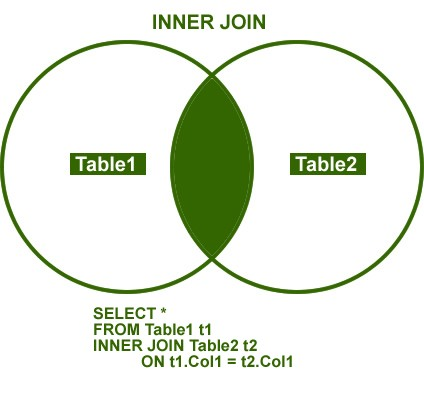
\includegraphics[width=0.5\textwidth]{logical_operators/inner_join.jpg}
\caption{An example about inner join.}
\end{figure}
 }
\vspace{0.5cm}
\subsubsection{Outer join}
{\justify
\begin{itemize}
{
\item Left outer join: The result  of a left outer join for tables A and B always contains all rows of the "left" table (A), even if the join-condition does not find any matching row in the "right" table (B). This means that if the {\bfseries ON} clause matches 0 rows in B (for a given row in A), the join will still return a row in the result (for that row) - but with NULL in each column from B. A left outer join returns all the values from an inner join plus all values in the left table that do not match to right table, including rows with NULL (empty) values in the link column.
\par }
{
\begin{figure}[H]
\centering
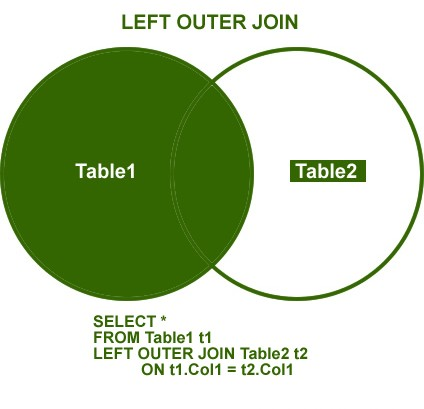
\includegraphics[width=0.5\textwidth]{logical_operators/left_outer_join.jpg}
\caption{An example about left outer join.}
\end{figure}
}
\vspace{0.5cm}
{
\item Right outer join: A right outer join (or right join) closely resembles a left outer join, except with the treatment of the tables reversed. Every row from the "right" table (B) will appear in the joined table at least once. If no matching row from the "left" table (A) exists, NULL will appear in columns from A for those rows that have no match in B. A right outer join returns all the values from the right table and matched values from the left table (NULL in the case of no matching join predicate).
\par }
{
\begin{figure}[H]
\centering
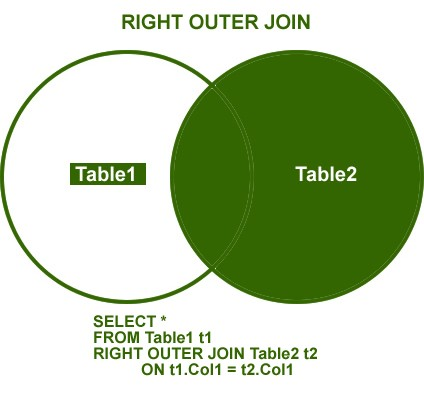
\includegraphics[width=0.5\textwidth]{logical_operators/right_outer_join.jpg}
\caption{An example about right outer join.}
\end{figure}
 }
\vspace{0.5cm}
{\justify
\item Full outer join: Conceptually, a full outer join combines the effect of applying both left and right outer joins. Where rows in the FULL OUTER JOINED tables do not match, the result set will have NULL values for every column of the table that lacks a matching row. For those rows that do match, a single row will be produced in the result set (containing columns populated from both tables).
\par }
{
\begin{figure}[H]
\centering
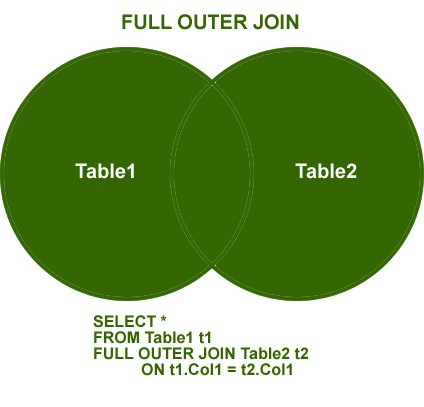
\includegraphics[width=0.5\textwidth]{logical_operators/full_outer_join.jpg}
\caption{An example about full outer join}
\end{figure}
 }
\vspace{0.5cm}
\end{itemize}
\par }
\vspace{0.5cm}
\subsubsection{Cross join}
{\justify
The SQL Cross join produces a result set which is the number of rows in the first table multiplied by the number of rows in the second table if no Where clause is used along with Cross join. If where clause is use with Cross join, it functions like an INNER JOIN
\par }
\vspace{0.5cm}
%Physical join operators
\subsection{Physical join operators}
{\justify
We use logical operators when we write queries to define a relational query at the conceptual level. To implement these logical join operators, DBMS use three different physical operators. Three physical join operators are respectively Nested Loops Join, Hash Join, Merged Join
\par }
\vspace{0.5cm}
\subsubsection{Nested Loops Join}
{\justify
A Nested Loops join \cite{physical operators} is a logical structure in which one loop (iteration) sedides inside another one, that is to say for each iteration of the outer loop all the iterations of the inner loop are executed/processed. To be more specific, For each row of the outer table, all the rows from the inner table are matched one by one if the row matches it is included in the result-set otherwise it is ignored. Then the next row from the outer table is picked up and the same process is repeated and so on.
\par }
\vspace{0.5cm}
{\justify
In terms of complexity, If we assume that N is the number of rows from the outer output and the number of rows that table is M. The complexity of this join operator is O(NlogM). Therefore, The PostgreSQL's optimizer might choose a Nested Loops join when  one of the joining tables is small (considered as the outer table) and another one is large (consider as the inner table which is indexed on the column that is in the join).
\par }
\vspace{0.5cm}
\subsubsection{Merge Join}
{\justify
The first thing about a Merge join \cite{physical operators} is that it requires both inputs to be sorted on join keys/merge columns (or both input tables have clustered indexes on the column that joins the tables). Because the rows are pre-sorted, a Merge join immediately begins the matching process. It reads a row from one input and then compares it with the row of another input. If the rows match, that matched row is considered in the result-set (then it reads the next row from the input table, does the same comparison/match) or else the lesser of the two rows is ignored and the process continues this way until all rows have been processed.
\par }
\vspace{0.5cm}
{\justify
In terms of complexity, If we assume that N is the number of rows from the outer output and the number of rows that table is M. The complexity of this join operator is O(N+M). If the inputs are not both sorted on the join key, the PostgreSQL optimizer will often choose the Merge join type due the the cost of pre-sorting process.
\par }
\vspace{0.5cm}
\subsubsection{Hash join.}
{\justify
A Hash join \cite{physical operators} is performed in two phases; the Build phase and the Probe phase and so the hash join has two inputs i.e, build input and probe input. The smaller of the input tables is considered as the build input and the other one is probe input
\par }
\vspace{0.5cm}
{\justify
During the build phase, joining keys of all the rows of the build table are scanned. Hashes are generated and placed in an in memory hash table. During the probe phase, joining keys of each row of the the probe table scanned. Again hashes are generated and compared against the corresponding hash table for a match. 
\par }
\vspace{0.5cm}
{\justify
A Hash function requires significant amount of CPU cycles to generate hashes and memory resources to store the hash table. If there is memory pressure, some of the partitions of the hash table are swapped to tempdb and whenever there is a need, it is brought back into cache. To achieve high performance, the PostgreSQL optimizer may parallelize a Hash join to scale better than any other join
\par }
\vspace{0.5cm}
{\justify
 In term of complexity, we’ll assume $h_c$ is the complexity of the hash table creation, and $h_m$ is the complexity of the hash match function. Therefore, the complexity of the Hash join will be O(N*$h_c$ + M*$h_m$ + J) where N is the smaller data set, M is the larger data set and J is a “joker” complexity addition for the dynamic calculation and creation of the hash function.
\par }
\vspace{0.5cm}
\section{BENCHMARKING.}
{\justify
I use JOB benchmark queries to examine the q-error of Postgresql estimator's cardinality estimation. The volume of JOB data set is about 20GB. Figure 4.5 shows the q-error of plan node by its join level. Figure 4.6 shows the q-error of plan node per query. Figure 4.7 and figure 4.8 show respectively the q-error of plan node by join tree depth, the actual execution time and estimated execution time of queries.
\par }
{
\begin{figure}[H]
\centering
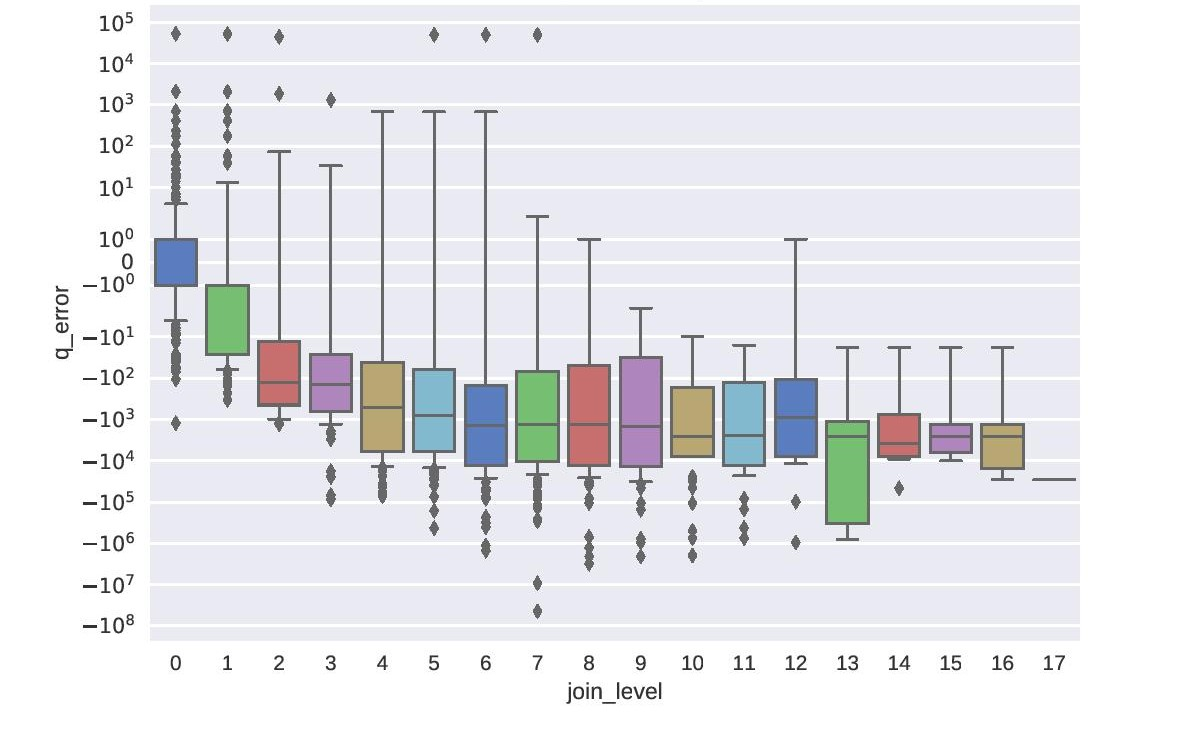
\includegraphics[width=1.0\textwidth]{results/plan_node_q-error.jpg}
\caption{Q-error of plan node and its join level.}
\end{figure}
}
{
\begin{figure}[H]
\centering
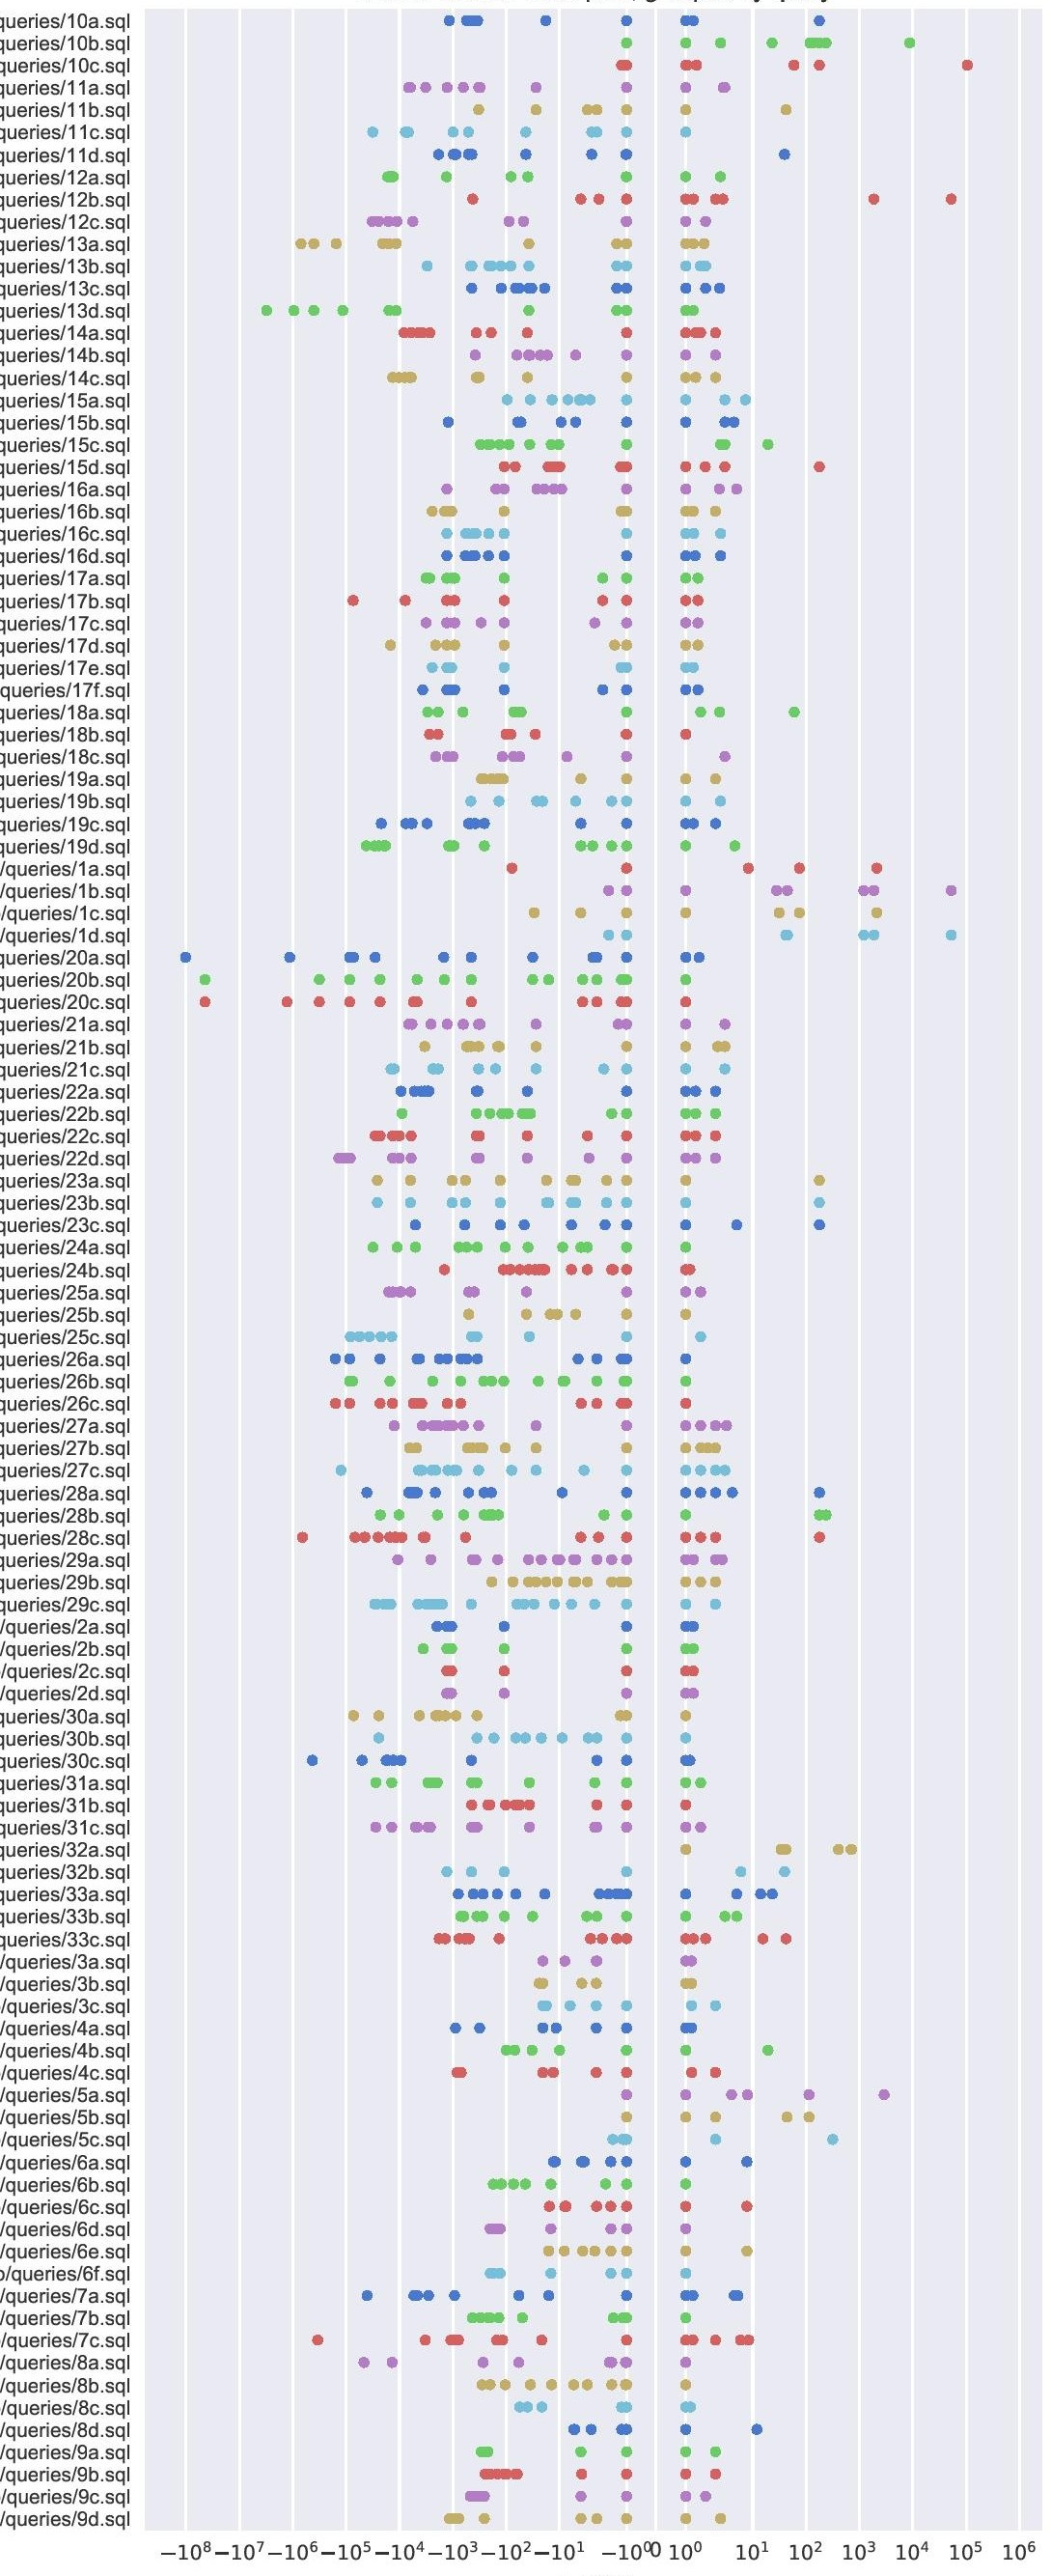
\includegraphics[width=0.59\textwidth]{results/q-error_per_query.jpg}
\caption{Q-error of plan node per query.}
\end{figure}
}
{
\begin{figure}[H]
\centering
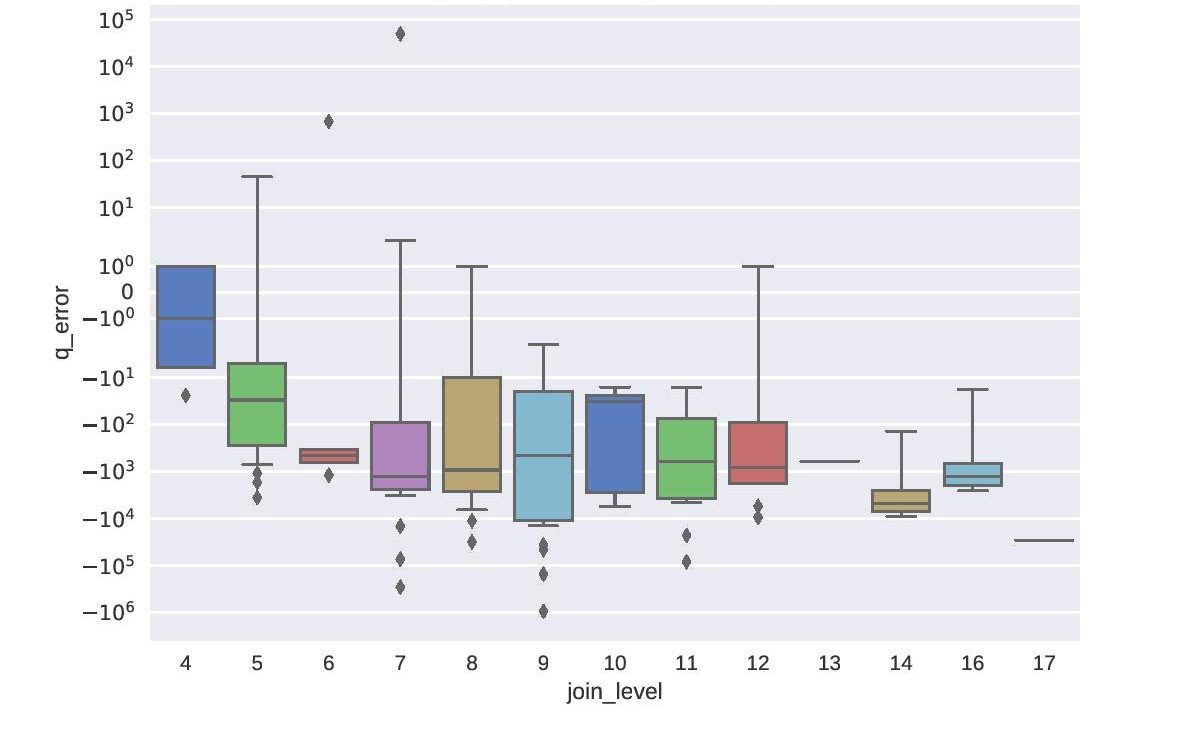
\includegraphics[width=1.0\textwidth]{results/plan_node_q-error_join_tree_depth.jpg}
\caption{Q-error of plan node and join tree depth.}
\end{figure}
}
{
\begin{figure}[H]
\centering
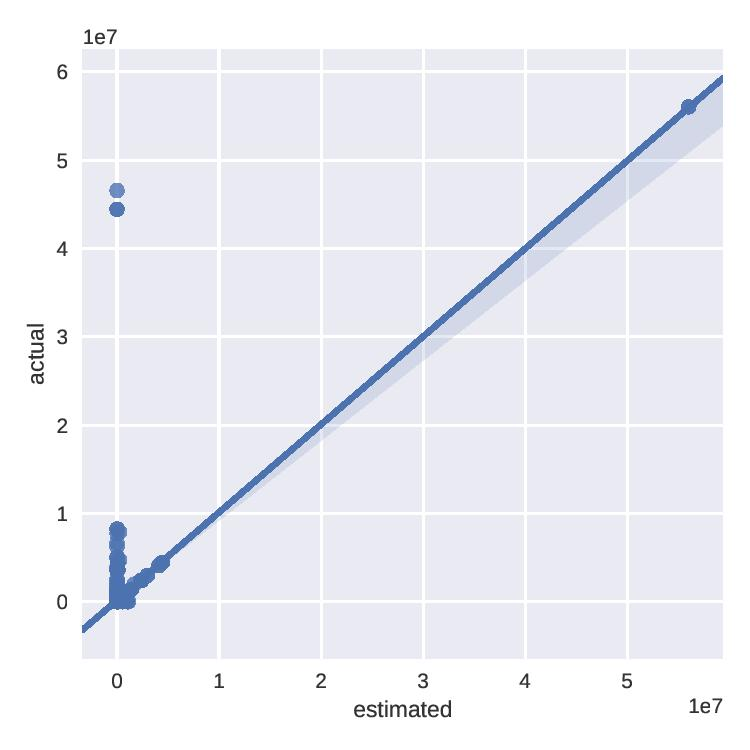
\includegraphics[width=1.0\textwidth]{results/actual_time_and_estimated_time.jpg}
\caption{actual execution time and estimated execution time.}
\end{figure}
}
%this section mentions the results of our extension.
\section{ANALYZING THE EFFECT OF BAD CARDINALITY ESTIMATION.} 
{\justify
As i mentioned in chapter 2, PostgreSQL optimizer is a purely cost-based optimizer. Therefore, when the cost is misestimated, it  leads to that PostgreSQL choose the plan which is not the best plan to execute. The example below shows the effect of estimation to choosing the plan of the PostgreSQL's optimizer :
\begin{itemize}
{
\item A, B are two relations; $card\left(A\right)_{est}$, $card\left(B\right)_{est}$ are respectively cardinality estimation of A,B; $card\left(A\right)_{real}$, $card\left(A\right)_{real}$ are respectively true cardinality of A, B.
\par }
{\centering $card\left(A\right)_{est}$ = 1000, $card\left(B\right)_{est}$ = 1 \\
$card\left(A\right)_{real}$ = 1000, $card\left(B\right)_{real}$ =  1000\\
}
\newpage
\begin{table}[ht]
\begin{center}
\begin{tabular}{|c|c|}
\hline
A nested loop join B  & A merge join B\\
\hline
complexity = O(n*m) & complexity = O(n+m)\\
\hline 
estimated cost = 1000 * 1 = 1000 & estimated cost = 1000 + 1 = 1001\\ 
\hline 
actual cost = 1000 * 1000 = 1000000 & actual cost = 1000 + 1000 = 2000\\ 
\hline 
\end{tabular}
\end{center}
\label{tab:dum1}
\caption{Operators sensitivity to estimation errors.}
\end{table}
{\justify
The underestimation of PostgreSQL's estimator in this example is 1000. Look at the table, we find that the estimated cost of nestedloop join is smaller than the estimated cost of merge join, so the planner's choice is nestedloop join instead of merge join whose actual cost is smaller about 1000 times than nestedloop join. 
\par}
\end{itemize}
\par}
{\justify
Figure 4.5, figure 4.6, figure 4.7, we find that most of the cardinality estimation of PostgreSQL estimator on JOB benchmark is underestimation. As a consequence of this underestimation, PostgreSQL's optimizer decides to introduce a nestedloop join because of a very low cardinality estimate, whereas in fact the true cardinality is larger, which lead PostgreSQL's optimizer to choose worse plan. To demonstrate the effect of this underestimation of PostgreSQL's estimator, i make the comparision between query performance between PostgreSQL with and without nestedloop join on JOB benchmarks. 
\par}
\vspace{0.5cm}
\newpage
{
\begin{figure}[H]
\centering
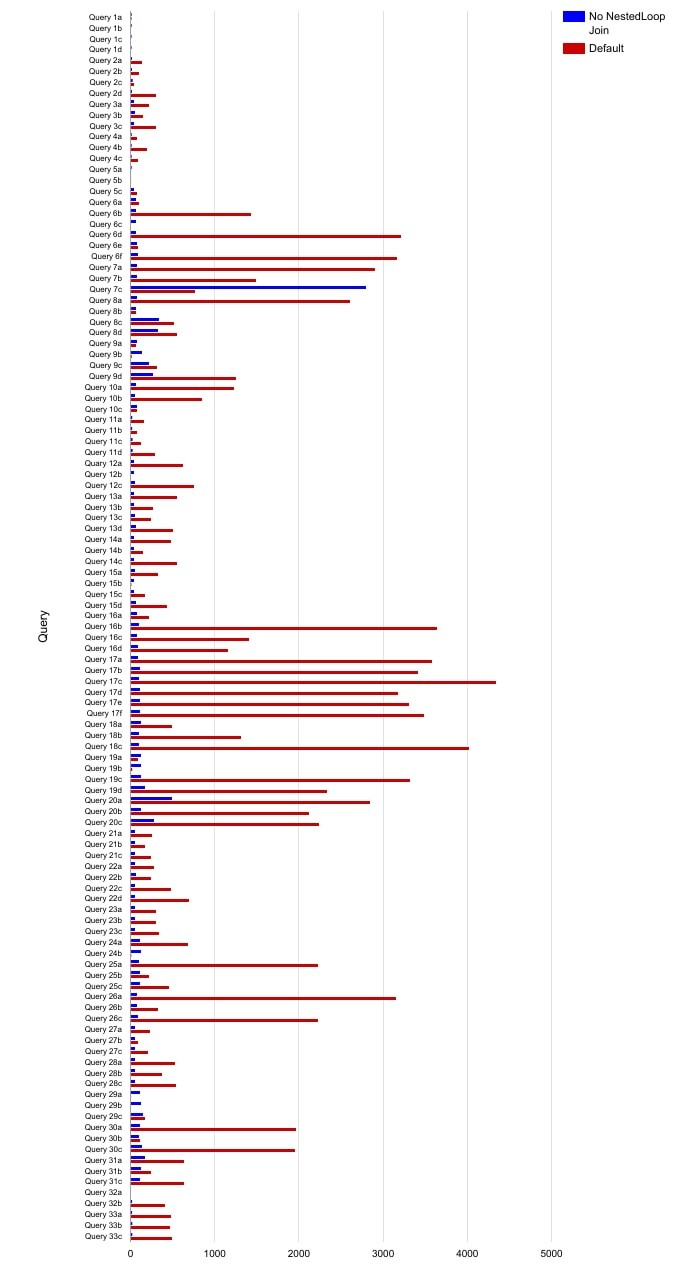
\includegraphics[width=0.77\textwidth]{results/execution_time_with_and_without_nestloop.jpg}
\caption{Query execution time (s) between  PostgreSQL with and without nestedloop join.}
\end{figure}
}
{\justify
As Firgure 4.9 shows, when rerunning all queries of JOB benchmarks without the risky nested-loop joins, we observed that the queries's execution time are improved significantly. For example, The execution time of query 6d is smaller 44 times after rerunning all queries of JOB benchmarks without the risky nested-loop joins, which increases from about 3213 seconds to nearly 73 seconds.
\par }
\section{THE PUBLISHED SOLUTIONS.}
{\justify
Today, there is no perfect solution for query optimization problem, so a lot of paper on existing algorithms improvement are published. There are different lines of research in query optimization field.
\begin{itemize}
\item Use machine learning methods for cardinality estimation. For example:
\begin{itemize}
\item In \cite{adaptive cardinality estimation} the main point of their approach is using query execution statistics of previously queries to improve cardinality estimations. It is called adaptive cardinality estimation.
\item In \cite{neural network approach} neural networks are used ti estunate the selectivity for user defined functions and data types. Nevertheless, this paper address the problem of estimation the selectivity for a single clause.
\item In \cite{probabilistic models} it is proposed to estimate node selectivity using inference in automatically constructed Bayesian networks. 
\end{itemize}
\item Use sampling-based approach \cite{sampling-based,cost models are unusable}. They do not improve query optimizer's cost estimator directly, but propose sampling-based ways to rectify standard query optimizer's errors if they are. Sampling-based approches are good on low-relational queries, but on queries with lots of joins they may have too large variance.
\item Use multidimensional statistics for correct cardinality estimation \cite{A multidimensional workload-aware histogram,multidimensional range queries}. The most popular kind of such statistics are multidimensional histograms. It is the most popular way to improve standard cardinality estimation method in DBMS community.
\end{itemize}
\par }
%this section is about our extension that i create for our benchmarking
%\section{Benchmarking extension}
%\begin{itemize}
%\item An extension makes the comparison between Postgresql, Postgresql with the true cardinality,Postgresql with some published solutions.
%\end{itemize}
%this section mentions about benchmarking with our extension
